\documentclass{standalone}

\usepackage{tikz}
\usetikzlibrary{positioning,arrows}

\begin{document}
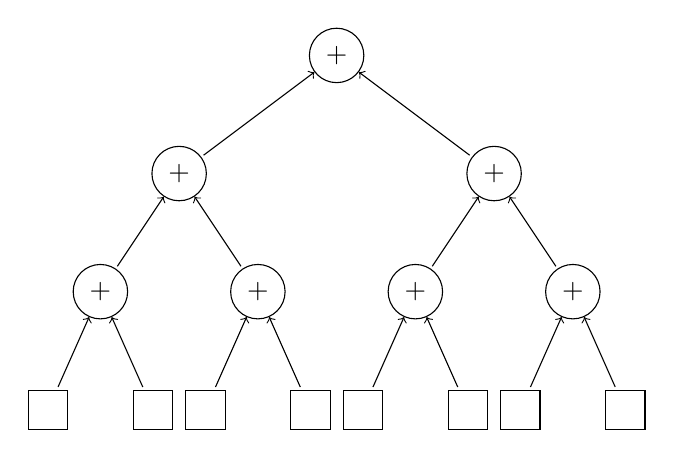
\begin{tikzpicture}[level/.style={sibling distance=40mm/#1},arrow/.style={draw=black, <-, shorten >=1pt}, edge from parent/.style={arrow}]
	\node[circle,draw] {+}
	child {node[circle,draw] {+}
			child {node[circle,draw] {+}
					child {node[rectangle,draw,inner sep=2.5mm] {}}
					child {node[rectangle,draw,inner sep=2.5mm] {}}
				}
			child {node[circle,draw] {+}
					child {node[rectangle,draw,inner sep=2.5mm] {}}
					child {node[rectangle,draw,inner sep=2.5mm] {}}
				}
		}
	child {node[circle,draw] {+}
			child {node[circle,draw] {+}
					child {node[rectangle,draw,inner sep=2.5mm] {}}
					child {node[rectangle,draw,inner sep=2.5mm] {}}
				}
			child {node[circle,draw] {+}
					child {node[rectangle,draw,inner sep=2.5mm] {}}
					child {node[rectangle,draw,inner sep=2.5mm] {}}
				}
		};
\end{tikzpicture}
\end{document}


